\section{First Data}

\begin{figure}[!h]
\begin{center}
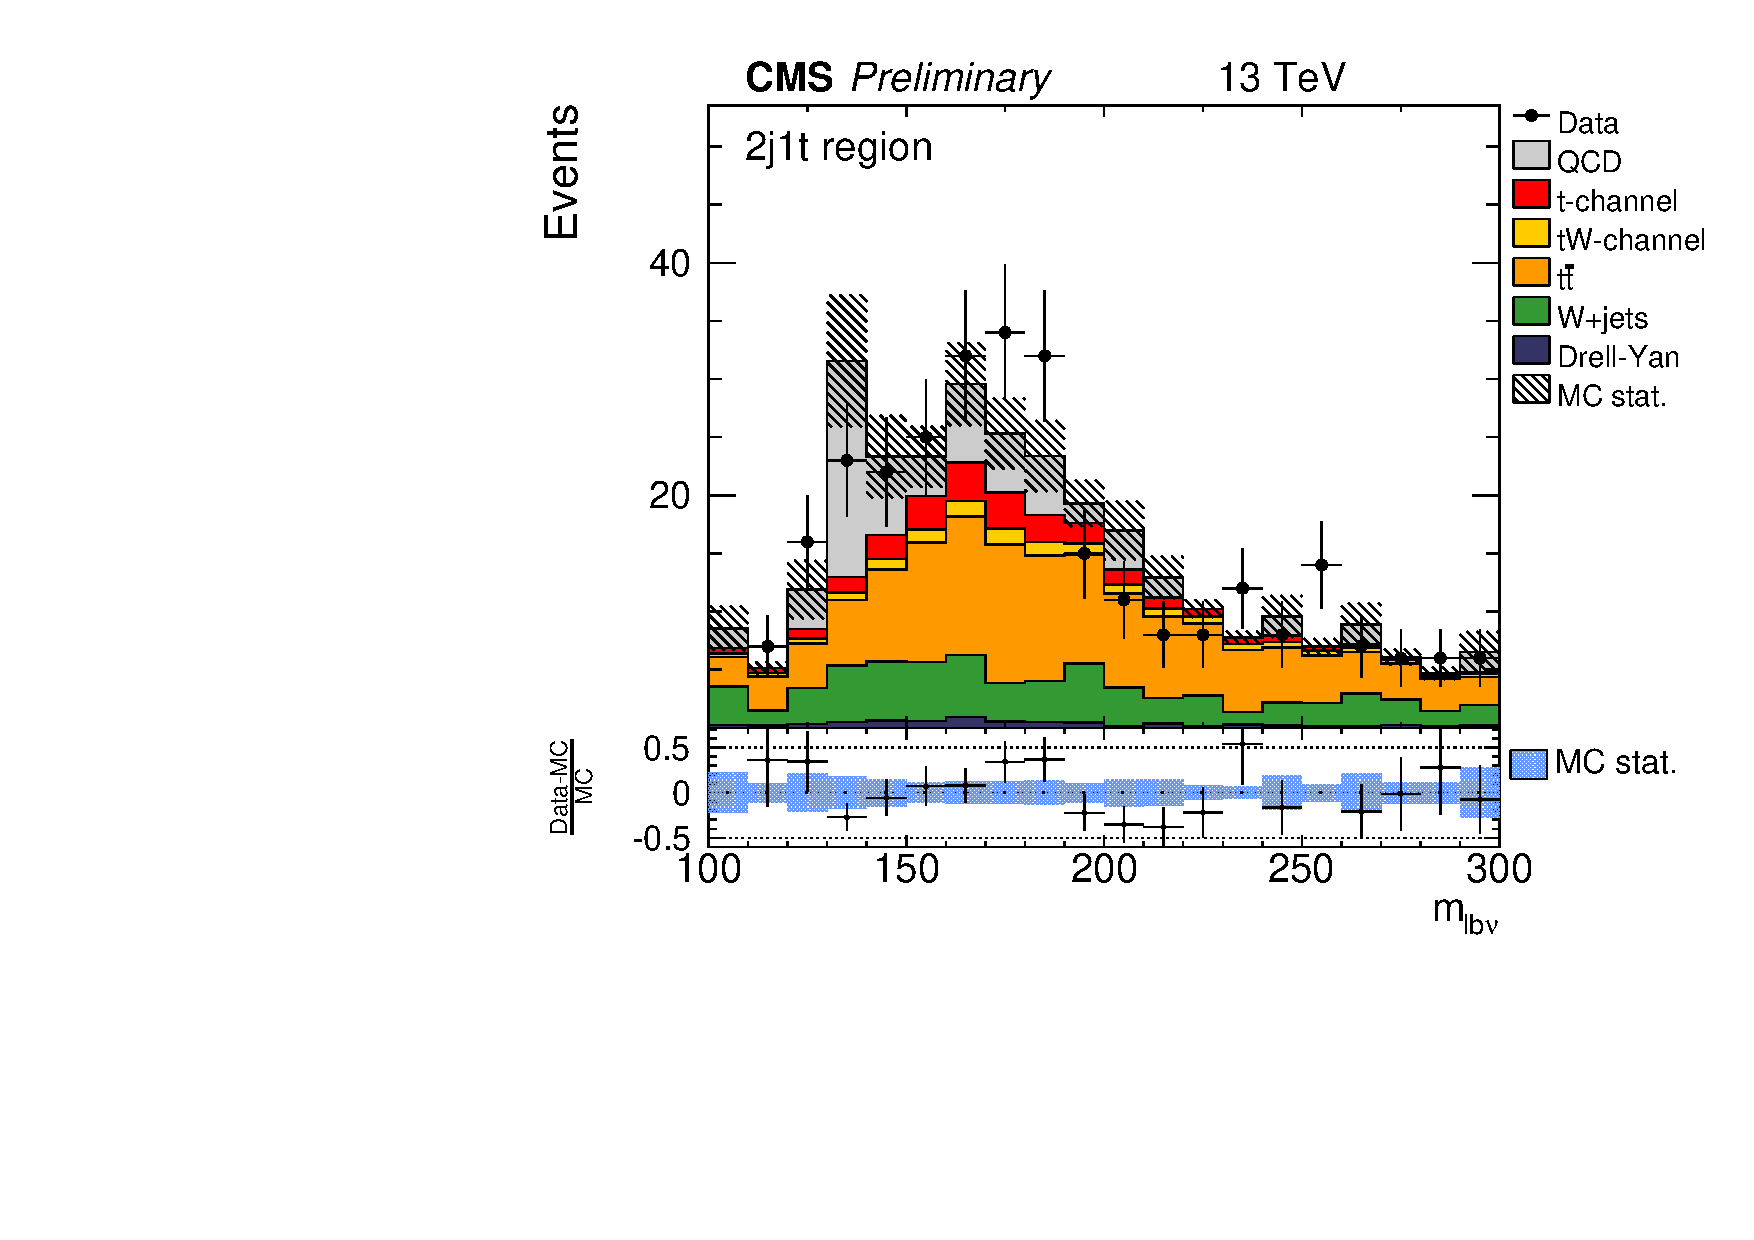
\includegraphics[angle=00,width=0.45\textwidth]{figures/DATA_2j1t_top_m.pdf}
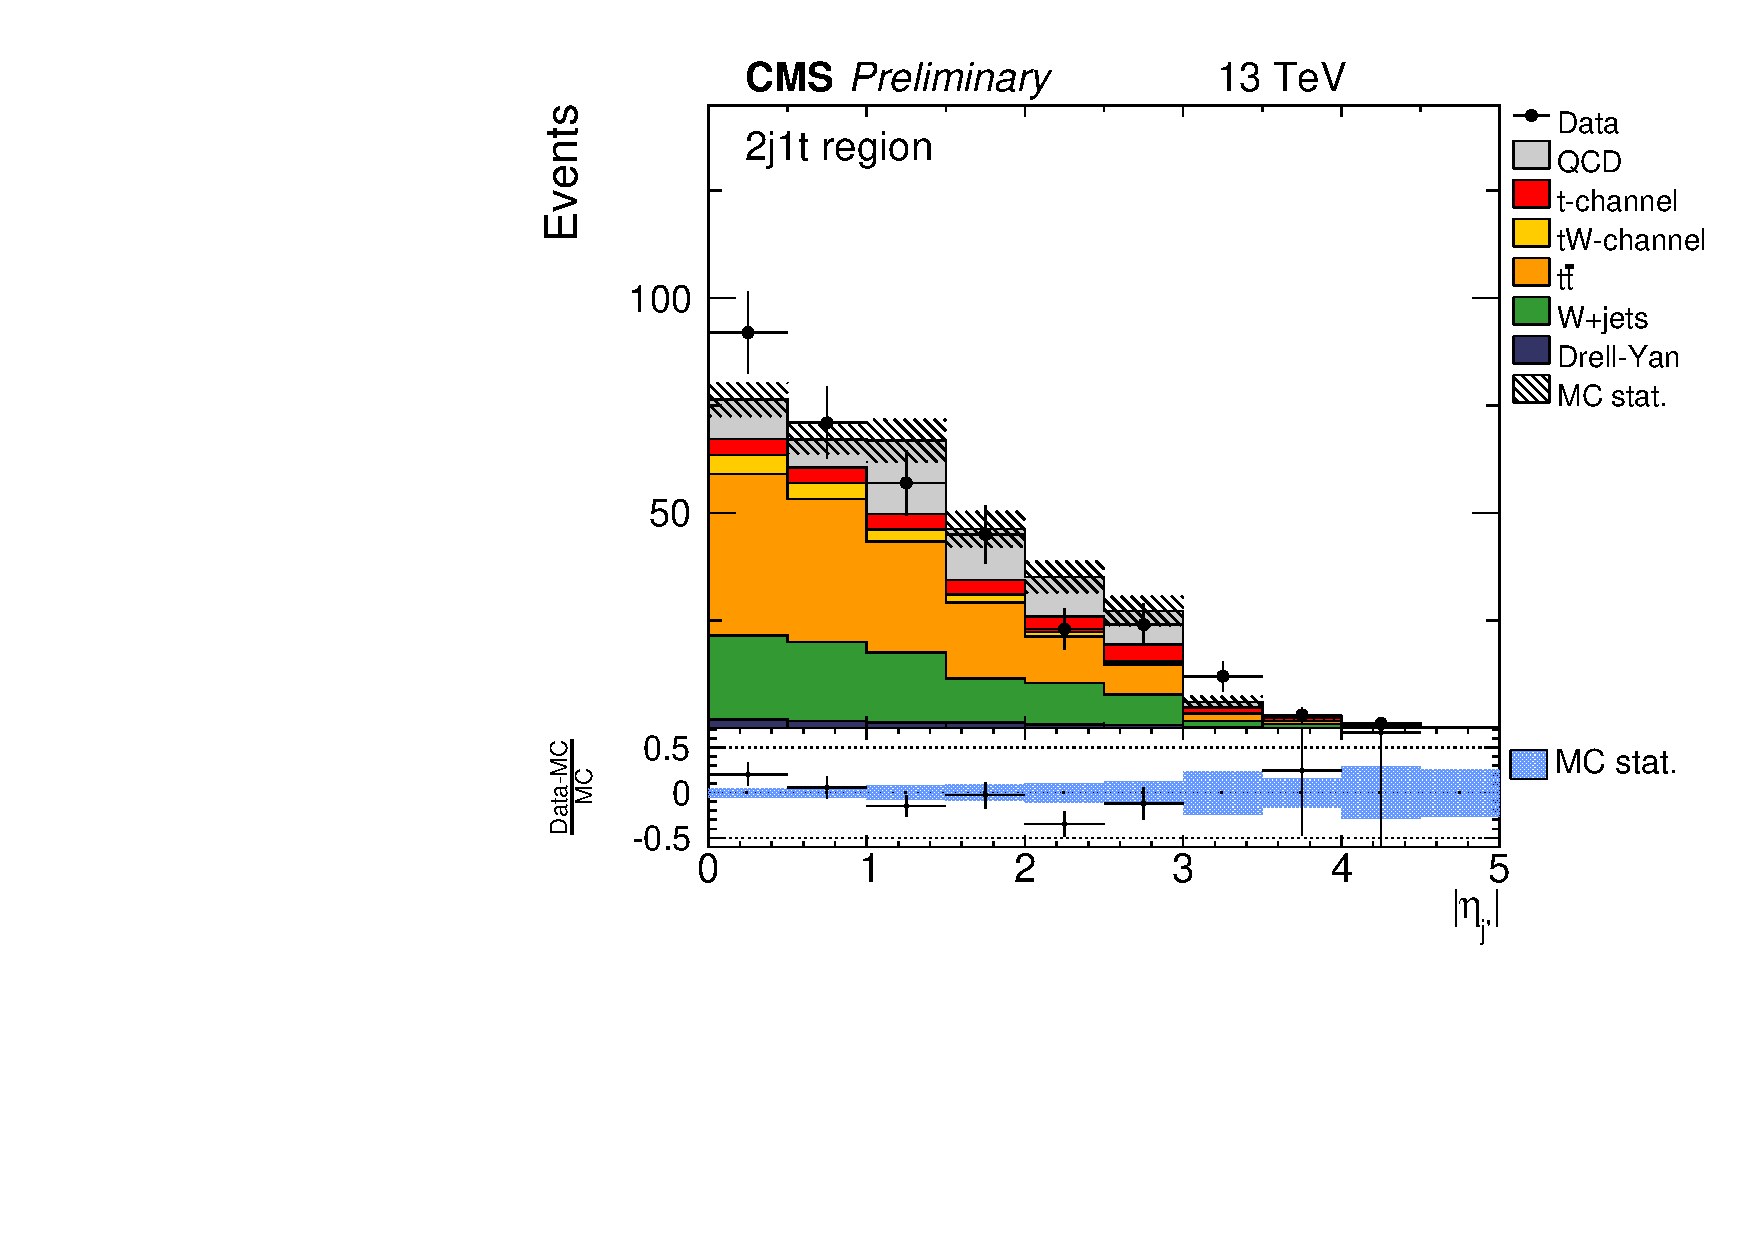
\includegraphics[angle=00,width=0.45\textwidth]{figures/DATA_2j1t_etajprime.pdf}\\
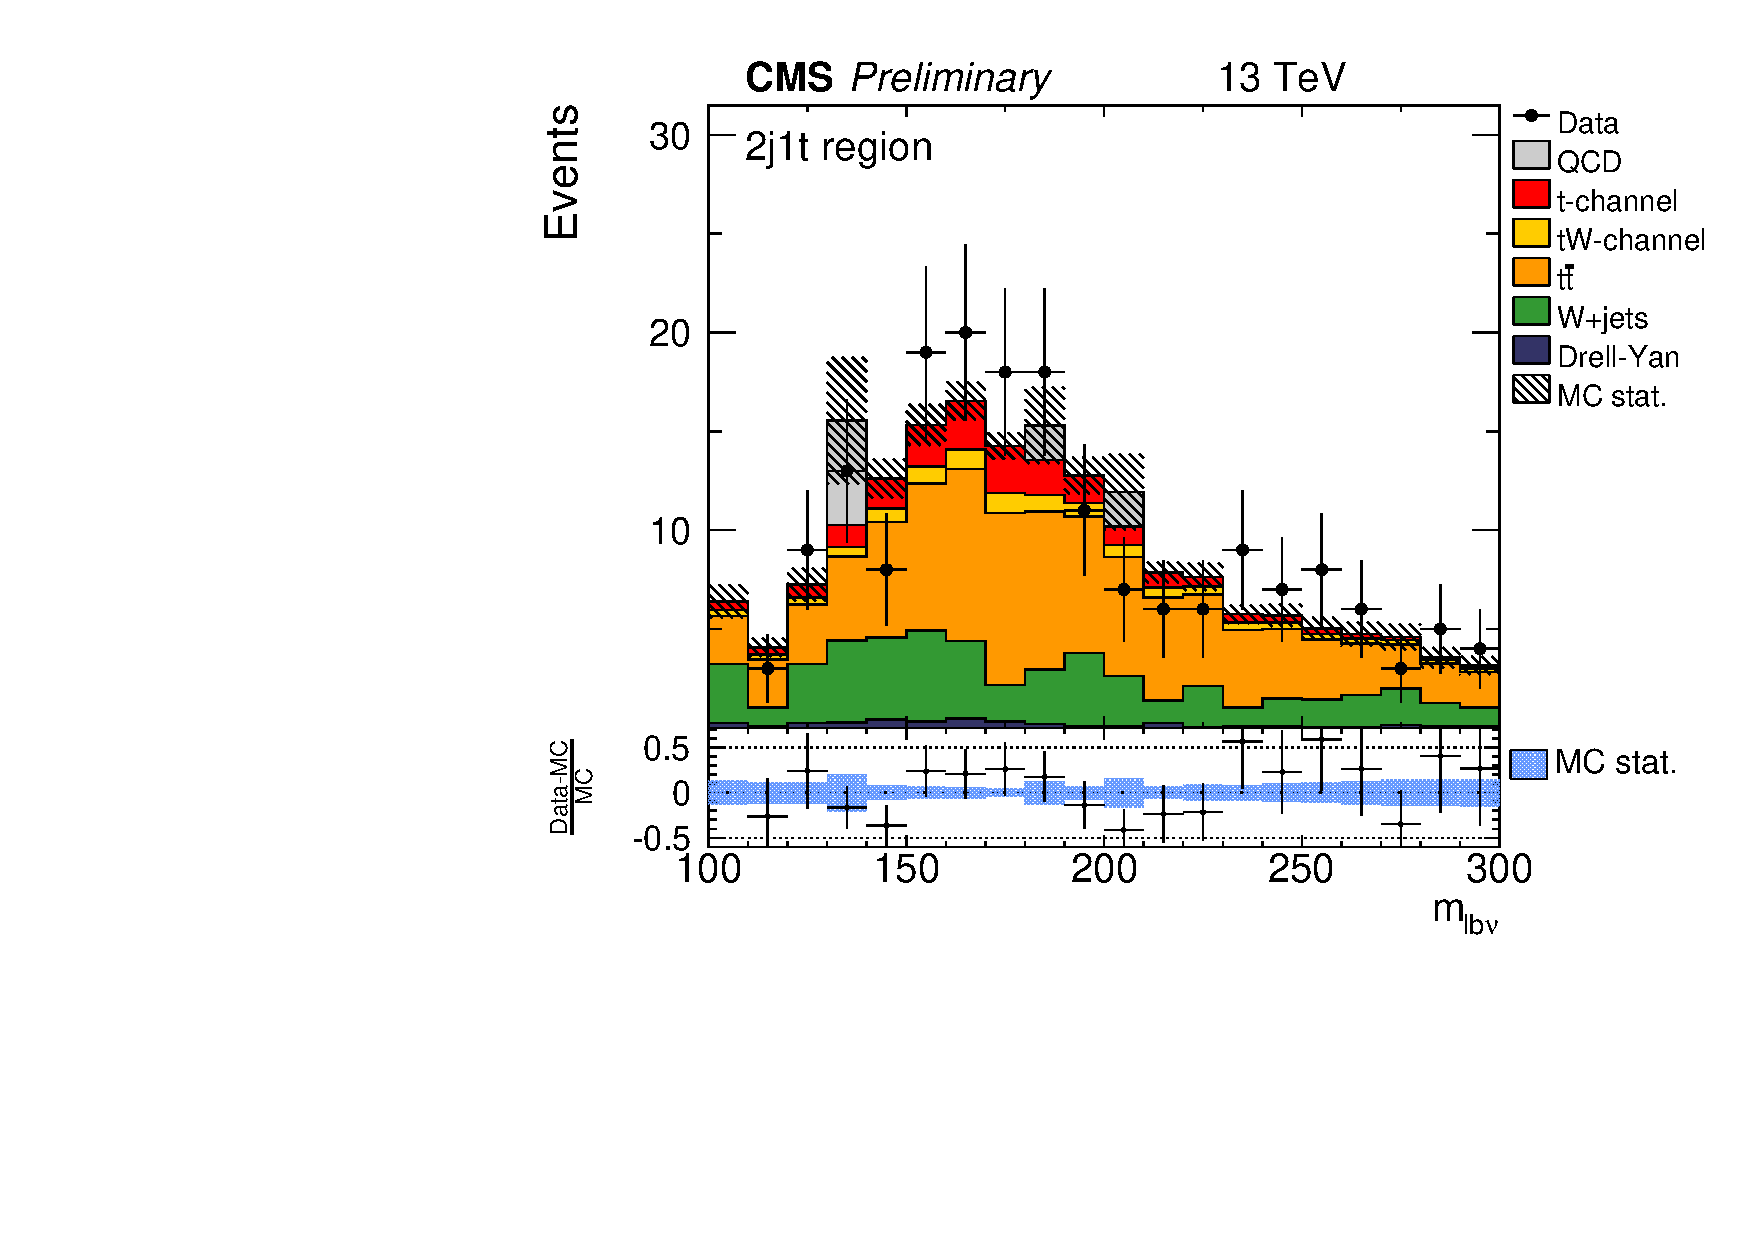
\includegraphics[angle=00,width=0.45\textwidth]{figures/DATA_2j1t_top_m_mtwcut.pdf}
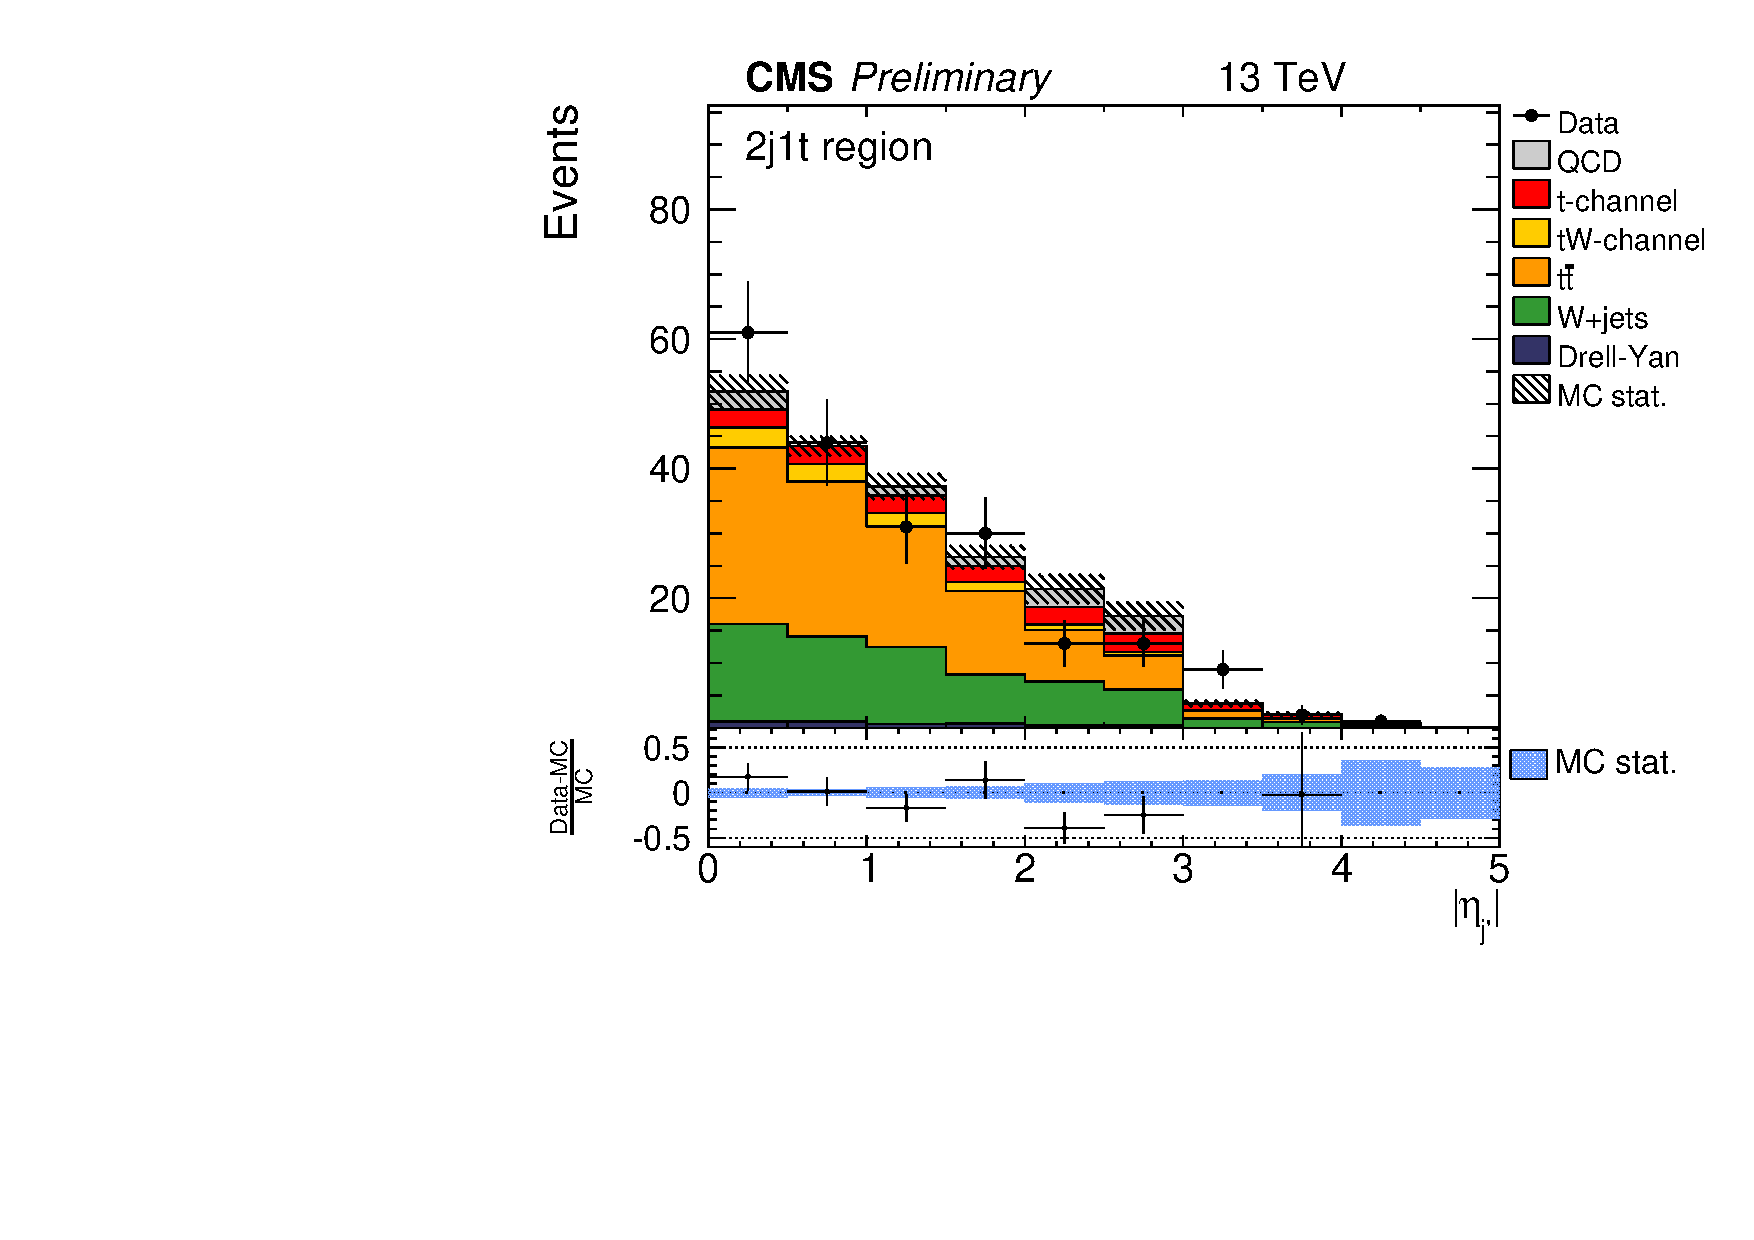
\includegraphics[angle=00,width=0.45\textwidth]{figures/DATA_2j1t_etajprime_mtwcut.pdf}
\caption{\label{aaa} Comparison of MC and the first Data from Run II. The left column shows the reconstructed top quarks mass and the right column the pseudorapidity of the light jet in the 2j1t region. An additional cut on $m_{\text{T,W}} > 50 \GeV$ is applied on the bottom row. MC is scaled to data.}
\end{center}
\end{figure}


